% Archivo principal: main.tex
\documentclass[12pt,letterpaper]{report}
%---------------------------------------------------------------------
% Paquetes
%---------------------------------------------------------------------
\usepackage[justification=centering]{caption}
\usepackage{multicol}
\usepackage{pdfpages}
%---------------------------------------------------------------------
% Importar configuración externa
%---------------------------------------------------------------------
% Archivo de configuración: configuracion.tex

% Configuración de márgenes
\usepackage[left=3.5cm, right=3cm, top=3cm, bottom=3cm]{geometry}

% Configuración de idioma y tipografía
\usepackage[spanish]{babel}
\usepackage[T1]{fontenc}
\usepackage{times} % Times New Roman
\usepackage{fontsize}
\usepackage{xcolor}
\usepackage{geometry}
\usepackage{graphicx}
\usepackage{tocloft}

\graphicspath{{./img/}}
% Configuración del interlineado
\renewcommand{\baselinestretch}{1.5} % Interlineado 1.5

% Configuración de numeración de páginas
\usepackage{fancyhdr}
\pagestyle{fancy}
\fancyhf{}
\rfoot{\thepage} % Número de página alineado a la derecha
\renewcommand{\headrulewidth}{0pt} % Eliminar línea de encabezado

% Definición de macros para datos del documento
\newcommand{\titulo}[1]{\def\Titulo{#1}}
\newcommand{\autor}[1]{\def\Autor{#1}}
\newcommand{\tutor}[1]{\def\Tutor{#1}}
\newcommand{\fecha}[1]{\def\Fecha{#1}}
\newcommand{\departamento}[1]{\def\Departamento{#1}}
\newcommand{\carrera}[1]{\def\Carrera{#1}}
% Definir comando para mostrar solo el año actual
\newcommand{\fechaActual}{\number\year}

\newcommand{\caratulaTapa}{
	\begin{titlepage}
		\begin{center}
			{\fontsize{18}{20}\selectfont UNIVERSIDAD CATÓLICA BOLIVIANA SAN PABLO SEDE TARIJA}\\[0.5cm]
			{\fontsize{16}{18}\selectfont DEPARTAMENTO DE \MakeUppercase{\Departamento}}
			
			{\fontsize{14}{16}\selectfont CARRERA DE \MakeUppercase{\Carrera}\\}
			\begin{figure}[h]
				\centering
				
\includegraphics[height=7cm]{ucbLOGO}
			\end{figure}
			{\fontsize{16}{18}\selectfont \MakeUppercase{\Titulo} }
			\vspace{1cm}
			
			{\fontsize{14}{16}\selectfont POSTULANTE: \MakeUppercase{\Autor}\\}
		\end{center}
		\vspace{0.2cm}
		{\fontsize{12}{14}\selectfont
			Trabajo de proyecto de grado \textcolor{red}{(lo que corresponda según Reglamento de modalidades de graduación)} presentado en consideración de la Universidad Católica Boliviana "San Pablo, como requisito para optar el Grado Académico de Licenciatura en \Carrera 
		}
	
		{\centering \fontsize{14}{16}\selectfont TARIJA-BOLIVIA\\\Fecha\\}
		
		
		\thispagestyle{empty} % Evita numeración en la portada
	\end{titlepage}
}

% Comando para generar la portada (sin numeración de página)
\newcommand{\caratulaContenido}{
	\begin{titlepage}
		\begin{center}
			{\fontsize{18}{20}\selectfont UNIVERSIDAD CATÓLICA BOLIVIANA SAN PABLO SEDE TARIJA}\\[0.5cm]
			{\fontsize{16}{18}\selectfont DEPARTAMENTO DE \MakeUppercase{\Departamento}}
			
			{\fontsize{14}{16}\selectfont CARRERA DE \MakeUppercase{\Carrera}\\}
			\begin{figure}[h]
				\centering
				
\includegraphics[height=7cm]{ucbLOGO}
			\end{figure}
			{\fontsize{16}{18}\selectfont \MakeUppercase{\Titulo} }
			\vspace{1cm}
			
			{\fontsize{14}{16}\selectfont POSTULANTE: \MakeUppercase{\Autor}\\TUTOR: \MakeUppercase{\Tutor}}
		\end{center}
		\vspace{0.2cm}
		{\fontsize{12}{14}\selectfont
			Trabajo de proyecto de grado \textcolor{red}{(lo que corresponda según Reglamento de modalidades de graduación)} presentado en consideración de la Universidad Católica Boliviana "San Pablo, como requisito para optar el Grado Académico de Licenciatura en \Carrera 
		}
	
		{\centering \fontsize{14}{16}\selectfont TARIJA-BOLIVIA\\\Fecha\\}
		
		
		\thispagestyle{empty} % Evita numeración en la portada
	\end{titlepage}
}

% Iniciar numeración desde la introducción
\newcommand{\iniciarNumeracion}{
    \setcounter{page}{1} % Reiniciar la numeración de páginas
    \pagestyle{fancy} % Usar el estilo "fancy"
    \fancyhf{} % Limpiar encabezados y pies de página
    \fancyfoot[R]{\thepage} % Colocar el número de página a la derecha
    \renewcommand{\headrulewidth}{0pt} % Eliminar la línea del encabezado
    \renewcommand{\footrulewidth}{0pt} % Eliminar la línea del pie de página
    % Redefinir el estilo 'plain' para las páginas de inicio de capítulo
    \fancypagestyle{plain}{%
      \fancyhf{}%
      \fancyfoot[R]{\thepage}%
      \renewcommand{\headrulewidth}{0pt}%
      \renewcommand{\footrulewidth}{0pt}%
    }
}
\newcommand{\configurarIndices}{
    % Líder de puntos para el índice general (capítulos, secciones y subsecciones)
    \renewcommand{\cftchapleader}{\cftdotfill{\cftdotsep}}
    \renewcommand{\cftsecleader}{\cftdotfill{\cftdotsep}}
    \renewcommand{\cftsubsecleader}{\cftdotfill{\cftdotsep}}
    
    % Líder de puntos para la lista de figuras
    \renewcommand{\cftfigleader}{\cftdotfill{\cftdotsep}}
    
    % Líder de puntos para la lista de tablas
    \renewcommand{\cfttableader}{\cftdotfill{\cftdotsep}}
}
%---------------------------------------------------------------------
% Definir datos del documento
%---------------------------------------------------------------------
\departamento{ciencias de la tecnología e innovación}
\titulo{TITULO DE TRABAJO (escrito en un letra mayúscula redactado en un máximo de 3 lineas alineado y justificado tamaño t16)}
\autor{Nombre del Autor}
\tutor{Nombre Tutor}
\fecha{\number\year}
\carrera{ingeniería mecatrónica}
%---------------------------------------------------------------------
% Ajustes de numeración y estilos de página
%---------------------------------------------------------------------
\setcounter{secnumdepth}{5}  % Hasta subparagraph numerado
\fancypagestyle{inicio}{
  \fancyhf{} % Limpia encabezados y pies
  % Define el encabezado a la izquierda tanto para páginas pares como impares
  \fancyhead[LO,LE]{Mi Encabezado Personalizado}
  \renewcommand{\headrulewidth}{0.4pt} % Línea de separación (opcional)
}
%---------------------------------------------------------------------
% Inicio documento
%---------------------------------------------------------------------
\begin{document}
	%---------------------------------------------------------------------
	% Portadas
	%---------------------------------------------------------------------
	\caratulaTapa
	\caratulaContenido
	\newpage
	\clearpage
	\pagestyle{empty}
	%---------------------------------------------------------------------
	% Insertar artículo IEEE (compilado por separado)
	%---------------------------------------------------------------------
	{
	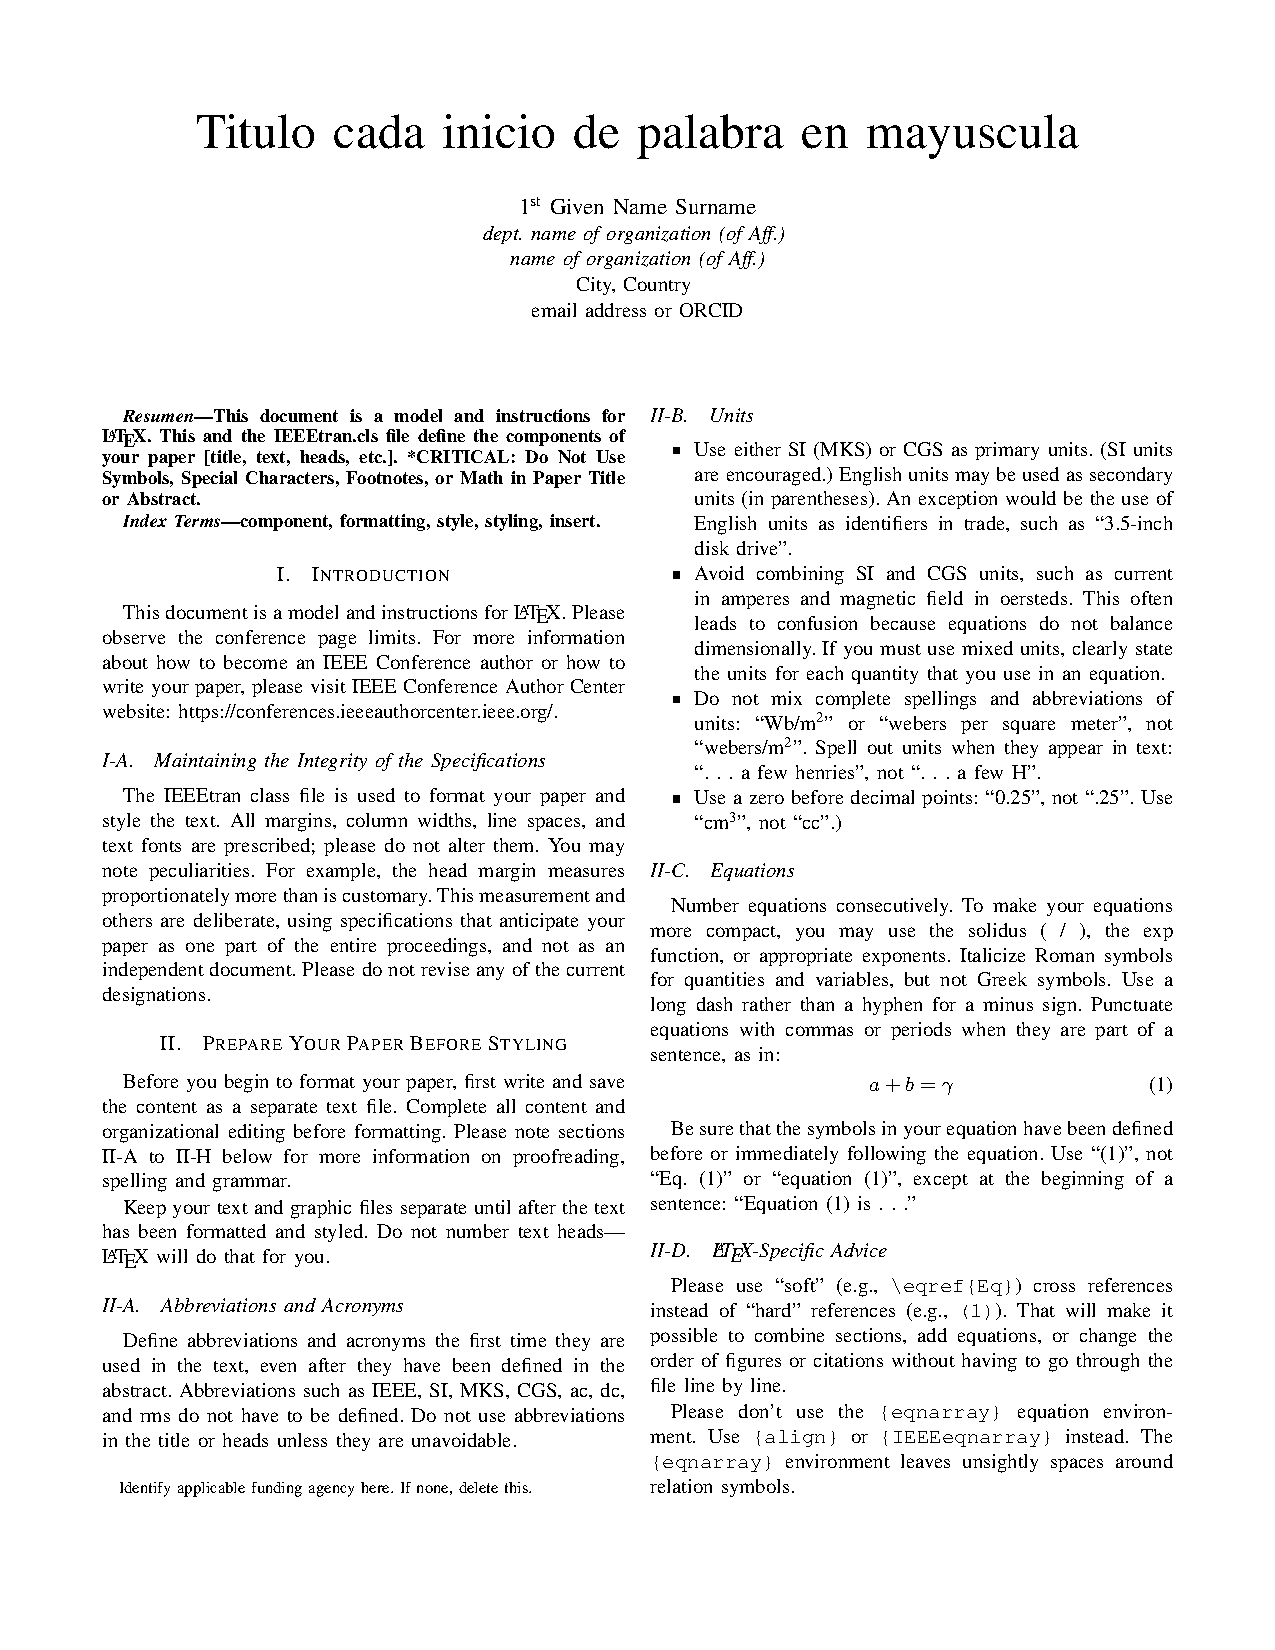
\includepdf[pages=-,scale=1]{IEEE/IEEE-conference-template-062824.pdf}
	}
	
	\newpage
	%---------------------------------------------------------------------
	% Resumen Ejecutivo
	%---------------------------------------------------------------------
	\begin{center}
	\section*{Resumen Ejecutivo}
	\end{center}
	Generalmente su extensión es igual a una plana, con una extensión de 150 a 200 palabras.\\
El mismo debe contener la información más importante de todo el trabajo, como:
breve descripción del problema, principales conclusiones o hallazgos del análisis,
principales características de la propuesta, y conclusiones del documento.\\
Al final del resumen se debe incluir entre tres (3) a cinco (5) palabras claves que
definen el contenido del trabajo.
	\thispagestyle{empty}
	\newpage
	%---------------------------------------------------------------------
	% Abstract
	%---------------------------------------------------------------------
	\begin{center}
	\section*{Abstract}
	Resumen Ejecutivo en formato inglés, siguiendo las misma estructura que el anterior apartado.
	
	\end{center}
	
	\thispagestyle{empty}
	\newpage
	
%---------------------------------------------------------------------
% Índices (índice general, figuras, tablas)
%---------------------------------------------------------------------
	\configurarIndices
    \tableofcontents
    \thispagestyle{empty}
    \newpage
    \listoffigures
    \thispagestyle{empty}
    \newpage
    \listoftables
    \thispagestyle{empty}
    \newpage
	
	%---------------------------------------------------------------------
	% Iniciar numeración normal
	%---------------------------------------------------------------------
	\iniciarNumeracion
	%---------------------------------------------------------------------
	% Secciones principales
	%---------------------------------------------------------------------
	\renewcommand{\thesection}{\arabic{section}}
	\begin{center}
	\section{Análisis del problema}
	\end{center}
	
	Aquí inicia el desarrollo del documento.
	\subsection{Introducción}
	Breve presentación del tema del proyecto y su relevancia
	\subsection{Descripción del problema}
	Detalle especifico del problema que se va a abordar, destacando su importancia.
	\subsection{Formulación del problema}
	Planteamiento claro y conciso del problema del proyecto.
	\subsection{Pregunta de investigación (opcional)}
	Pregunta principal que el proyecto busca responder.
	\subsection{Objetivos del proyecto}
	\textcolor{red}{
	\begin{itemize}
	\item \textbf{Generales: }expresan las intenciones educativas de un proyecto curricular, de un plan
de estudios, o de una asignatura. Son los propósitos más amplios que persigue un
programa en cada nivel y su cumplimiento está en función del tiempo de duración de
la carrera o de la asignatura dentro de la estructura y organización curricular.
	\item 
	\textbf{Particulares:} se derivan de los generales de la asignatura y corresponden a cada una
de las unidades del programa analítico de la misma. Aquí se precisan las intenciones
educativas de una parte del contenido (sistema de conocimientos y sistema de
habilidades), que se aborda, lo cual debe conducir al logro de los objetivos generales
de la asignatura en su conjunto y de los objetivos curriculares del Plan de Estudios.
	\item 
	\textbf{Específicos:} se derivan de los objetivos particulares y corresponden a los de las clases
de cada unidad didáctica, por lo que existe un mayor grado de concreción de las
intenciones educativas. El cumplimiento de estos objetivos debe conducir al logro de
los objetivos de la unidad del programa de la asignatura, como parte de la estructura
curricular y contribuir al cumplimiento de los objetivos del plan de estudio.
	\end{itemize}	
	¿CÓMO REDACTAR OBJETIVOS?\\
1. Todo objetivo inicia su redacción utilizando un verbo en forma infinitiva, así se
precisa el propósito del objetivo con más claridad. Este verbo describe el qué del
objetivo.Por ejemplo:\\
Identificar …………\\
Comparar …………\\
Aplicar ……………\\
Diagnosticar …………\\
Describir ………\\
Reflexionar……………\\
Fundamentar …………\\
2. Para completar el enunciado del objetivo se da respuesta al PARA QUE del
propósito. Es decir se explica la finalidad del objetivo. Por ejemplo:\\
… con el fin de ….\\
…. para….\\
3. Termina enuciando el CÓMO se logrará el objetivo. Por ejemplo:\\
…………mediante ….\\
……… a través de …..\\
…….. utilizando …..\\
	}
	
	

	


	\subsubsection{Objetivo general}
	Meta  del proyecto.
	\subsubsection{Objetivos específicos}
	Metas secundarias que ayudan a alcanzar el objetivo general.
	\subsection{Delimitación del proyecto}
	Definición del alcance y las limitaciones del estudio.
	\subsection{Justificación}
	Explicación de la relevancia y la importancia del proyecto, y como contribuirá al campo tecnológico.
	
	%---------------------------------------------------------------------
	% Marco Teórico
	%---------------------------------------------------------------------
	\newpage
	\begin{center}
	\section{Marco Teórico}
	\end{center}
	\subsection{Antecedentes y referencias}
	Información previa y estudios anteriores relevantes al tema del proyecto.
	\subsection{Estado del arte}
	Resumen y análisis de las investigaciones mas recientes y relevantes en el área, identificando tendencias y vacíos en el conocimiento.
	\subsection{Desarrollo de teorías y modelos}
	Descripción de las teorías y modelos que sustentan el proyecto.
	\subsection{Definición de términos básicos}
	Explicación de términos técnicos y conceptos específicos utilizados en el proyecto
	
	%---------------------------------------------------------------------
	% Marco Tecnológico
	%---------------------------------------------------------------------
	\newpage
	\begin{center}
	\section{Marco tecnológico}
	\end{center}
	
	\subsection{Tecnologías utilizadas y tendencias}
	Identificación de tecnologías, sus tendencias y su impacto potencial en el proyecto.
	
	\subsection{Comparación de tecnologías}
	Análisis comparativo de diferentes tecnologías disponibles.
	
	%---------------------------------------------------------------------
	% Marco Metodológico
	%---------------------------------------------------------------------
	\newpage
	\begin{center}
	\section{Marco metodológico}
	\end{center}
	
	\subsection{Metodología}
	Descripción detallada del enfoque y métodos utilizados para llevar a cabo el proyecto, incluyendo técnicas de recolección de datos y análisis.
	
	\subsection{Plan de trabajo}
	Cronograma y fases del proyecto, especificando actividades y tiempos estimados para cada etapa.
	
	%---------------------------------------------------------------------
	% Marco Legal (opcional)
	%---------------------------------------------------------------------
	\newpage
	\begin{center}
	\section{Marco legal (opcional)}
	\end{center}
	
	%---------------------------------------------------------------------
	% Ingeniería del Proyecto
	%---------------------------------------------------------------------
	\newpage
	\begin{center}
	\section{Ingeniería del proyecto}
	\end{center}
	
	%---------------------------------------------------------------------
	% Conclusiones y Recomendaciones
	%---------------------------------------------------------------------
	\newpage
	\begin{center}
	\section{Conclusiones y recomendaciones}
	\end{center}
	
	%---------------------------------------------------------------------
	% Bibliografía
	%---------------------------------------------------------------------
	\newpage
	\begin{center}
	\section*{Bibliografía}
	\end{center}
	Aquí van las referencias en formato APA 7ma edición.
	
	%---------------------------------------------------------------------
	% Anexos
	%---------------------------------------------------------------------
	\newpage
	\begin{center}
	\section*{Anexos}
	\end{center}
	Aquí se pueden agregar anexos.
	
	\begin{figure}[ht]
		
		% Incrementa el contador de figuras para numerarlas automáticamente
		\refstepcounter{figure}
		% Número de la figura en negrita
		\textbf{Figura \thefigure}\\[0.5em]
		% Título de la figura en cursiva (una línea debajo del número)
		\textit{Título breve pero descriptivo de la imagen}\\[1em]
		\begin{center}
			
			
\includegraphics[width=0.8\textwidth]{eje1.png}\\[1em]
		\end{center}
		% Inserción de la imagen
		
		% Leyenda: explicación de símbolos o detalles de la imagen
		
		% Nota: información adicional si fuese necesaria
		\normalsize Nota: Se incluye la nota únicamente cuando es necesaria para aclarar información adicional.
		\addcontentsline{lof}{figure}{Figura \thefigure. \textit{Título breve pero descriptivo}}
				
	\end{figure}
	
	\begin{table}[ht]
		\captionsetup{justification=raggedright,singlelinecheck=false}
		% -- La 'caption' define el título que aparecerá en el índice de tablas.
		% -- En estilo APA 7, normalmente se pone el número de tabla en negrita
		%    y debajo (o en la misma línea) el título en cursiva.
		\caption{\textit{Relación de variables en estudio}}
		\label{tab:variables} % Para referenciarla con \ref{tab:variables}
		\centering
		\begin{tabular}{l c}
			\hline
			\textbf{Variable} & \textbf{Valor} \\
			\hline
			Variable A        & 10 \\
			Variable B        & 20 \\
			\hline
		\end{tabular}
		
		% -- Nota al pie de la tabla, en flushleft, según convención APA (pequeña explicación).
		\begin{flushleft}
			\textit{Nota}. Ejemplo de tabla en estilo APA 7. * p < .05.  
			Los datos se obtuvieron de la base de datos interna.
		\end{flushleft}
	\end{table}
	\begin{table}[ht]
		\captionsetup{justification=raggedright,singlelinecheck=false}
		% -- La 'caption' define el título que aparecerá en el índice de tablas.
		% -- En estilo APA 7, normalmente se pone el número de tabla en negrita
		%    y debajo (o en la misma línea) el título en cursiva.
		\caption{\textit{Radelación de variables en estudio}}
		
		\centering
		\begin{tabular}{l c}
			\hline
			\textbf{Variable} & \textbf{Valor} \\
			\hline
			Variable A        & 10 \\
			Variable B        & 20 \\
			\hline
		\end{tabular}
		
		% -- Nota al pie de la tabla, en flushleft, según convención APA (pequeña explicación).
		\begin{flushleft}
			\textit{Nota}. Ejemplo de tabla en estilo APA 7. * p < .05.  
			Los datos se obtuvieron de la base de datos interna.
		\end{flushleft}
	\end{table}
\end{document}